\documentclass[tikz,border=6pt]{standalone}
\usepackage{tikz}
\usetikzlibrary{arrows.meta,positioning}
\definecolor{nebula}{HTML}{6366F1}
\definecolor{spark}{HTML}{14B8A6}
\definecolor{ink}{HTML}{334155}
\begin{document}
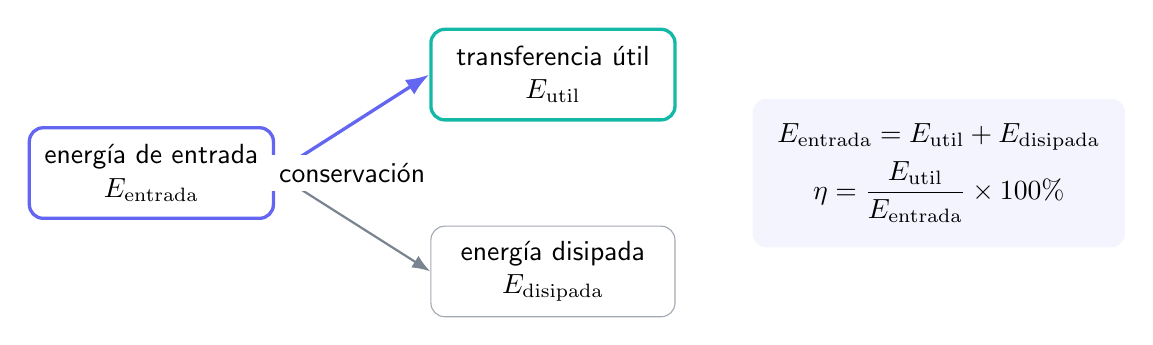
\begin{tikzpicture}[font=\sffamily,>=Latex,box/.style={draw=ink!45,rounded corners=5pt,minimum width=3.1cm,minimum height=1.15cm,align=center,fill=white}]
  \node[box,draw=nebula,very thick] (input) at (0,0) {energ\'ia de entrada\\$E_{\rm entrada}$};
  \node[box,draw=spark,very thick] (useful) at (5.1,1.25) {transferencia \'util\\$E_{\rm util}$};
  \node[box] (waste) at (5.1,-1.25) {energ\'ia disipada\\$E_{\rm disipada}$};
  \draw[->,very thick,nebula] (input.east)--(useful.west);
  \draw[->,thick,ink!65] (input.east)--(waste.west);
  \node[fill=white,inner sep=3pt] at (2.55,0) {conservaci\'on};
  \node[align=center,fill=nebula!7,rounded corners=5pt,inner sep=9pt] at (10.0,0) {$E_{\rm entrada}=E_{\rm util}+E_{\rm disipada}$\\[3pt]$\displaystyle \eta=\frac{E_{\rm util}}{E_{\rm entrada}}\times100\%$};
\end{tikzpicture}
\end{document}
